\section{Motivation}
\textbf{
    \begin{itemize}
        \item This should be discussed as an extension to the previous study.
        \item The plots should show the proportional relationship between hit efficiency and reconstruction efficiency.
        \item Discuss why it is important to recover tracks (high intensity experiment etc)
    \end{itemize}
}
In the Mu3e experiment the number of tracks recorded is directly proportional to the ratio between the number of hits that should be recorded in the silicon detector and the number of hits actually recorded. 
Figure \ref{fig:hit_eff} shows the relationship between the reconstruction efficiency and the hit efficiency. Whereby the hit efficiency is defined as the ratio between the number of hits recorded in the detector and the number of Monte Carlo (MC) truth hits. The reconstruction efficiency is defined as the number of tracks recorded normalised by the number of tracks recorded at $100\%$ hit efficiency.
\begin{figure}
    \centering
    \begin{subfigure}{.5\textwidth}
        \centering
        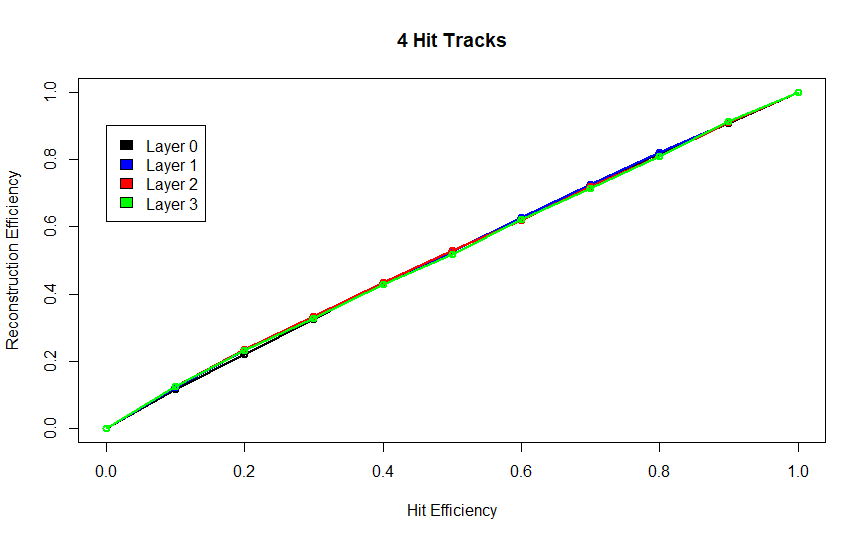
\includegraphics[scale=0.3]{fig/eff/4.png}
        \caption{Plots showing the relation between reconstruction efficiency and the hit efficiency.}
        \label{fig:eff4}
    \end{subfigure}%
    \begin{subfigure}{.5\textwidth}
        \centering
        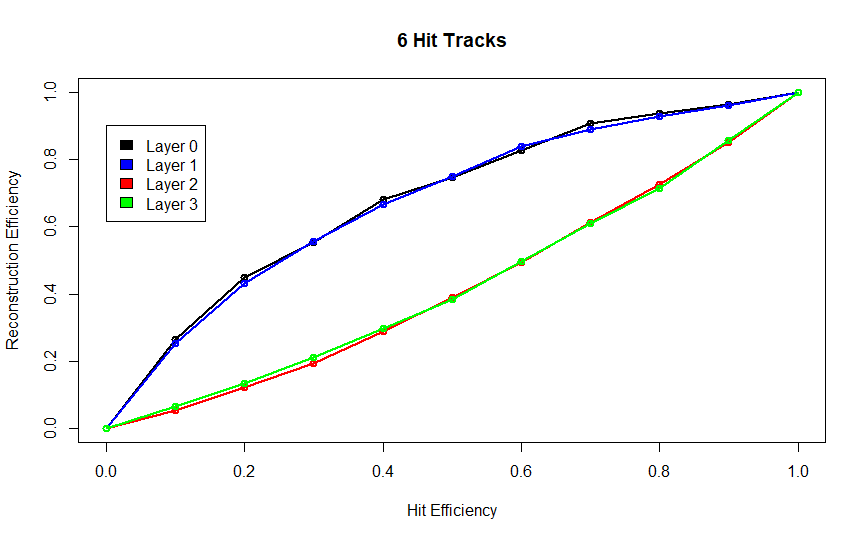
\includegraphics[scale=0.3]{fig/eff/6.png}
        \caption{Plots showing the relation between reconstruction efficiency and the hit efficiency.}
        \label{fig:eff6}
    \end{subfigure}
    \caption{The above figures show the effect a given hit efficiency has on the reconstruction efficiency for tracks that are both 4 and 6 hits long. Hit efficiency is defined as the ratio between the number of hits recorded in the detector and the total number of Monte Carlo hits. Reconstruction is defined as the total number of tracks generated at a given hit efficiency divided by the number of tracks generated with 100\% hit efficiency.}
    \label{fig:hit_eff}
\end{figure}
\section{Ordering of the Algorithm}
\textbf{
    \begin{itemize}
        \item You should use the top flowchart but redesign it in latex
        \item The number of subsections after this should be reduced.
    \end{itemize}
}
In this section, the order of the algorithm is discussed. 
Seen below is a flowchart where the order of the algorithm is summarised.
\par
\begin{figure}
    \centering
    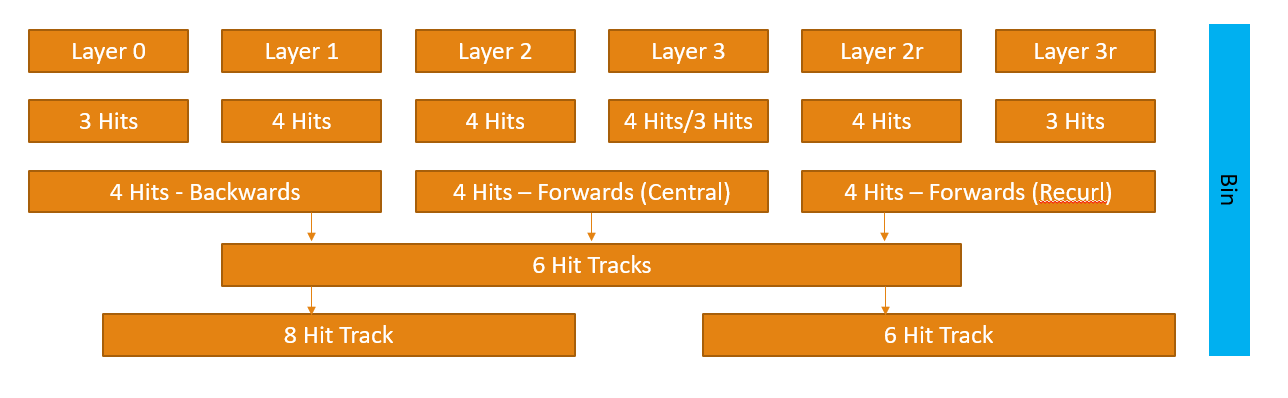
\includegraphics[scale=0.6]{fig/tracking/flow.png}
    \caption{This might be a better flowchart.}
    \label{fig:alt_flow}
\end{figure}
\usetikzlibrary{arrows,positioning,shapes.geometric}
    \begin{tikzpicture}[>=latex']
        \tikzset{block/.style= {draw, rectangle, align=center,minimum width=2cm,minimum height=1cm},
        rblock/.style={draw, shape=rectangle,rounded corners=1.5em,align=center,minimum width=2cm,minimum height=1cm},
        input/.style={ % requires library shapes.geometric
        draw,
        trapezium,
        trapezium left angle=60,
        trapezium right angle=120,
        minimum width=2cm,
        minimum height=1cm
    },
        }
        \node [block]  (start) {Run the Simulation and \\ Collect Hits in Layers};
        \node [block, right =1cm of start] (acquire) {Sort Hits into Frames};
        \node [block, right =1cm of acquire] (rgb2gray) {Map Hit Information: \\ Positional and Temporal};
        \node [block, below =1.5cm of start] (otsu) {Make Initial Triplets \\ for Each Layer: Link $\xrightarrow{}$ \ref{tab:1}};
        \node [block, right =1cm of otsu] (gchannel) {Divide each list of triplets into \\ smaller momentum ranges: Link $\xrightarrow{}$ \ref{2}};
        \node [rblock, right =1cm of gchannel] (closing) {Connect triplets together \\ from the Layer 2 triplets:  \\ Link $\xrightarrow{}$ \ref{3}};
        \node [block, below =1.5cm of otsu] (hit) {Make 4 hit tracks from triplets \\ before and after layer 2: Link $\xrightarrow{}$ \ref{4}};
        \node [block, right =1cm of hit] (hits) {Connect tracks together for \\ 6 hit tracks: Link $\xrightarrow{}$ \ref{5}};
        \node [block, below=1.5cm of hits] (limit) {Connect 6 hit tracks for 8 \\ hit tracks: Link $\xrightarrow{}$ \ref{6}};
        \node [coordinate, below right =0.75cm and 0.6cm of rgb2gray] (right) {};  %% Coordinate on right and middle
        \node [coordinate,above left =0.75cm and 0.6cm of otsu] (left) {};  %% Coordinate on left and middle  %% Coordinate on right 
  %% Coordinate on left and middle
        \node [coordinate, below right =0.75cm and 0.6cm of hits] (right3) {};  %% Coordinate on right and middle
        \node [coordinate,above left =0.75cm and 5.5cm of limit] (left3) {};  %% Coordinate on left and middle
        \node[coordinate, below = 0.75cm of closing] (right2){};
        \node[coordinate, above left = 0.75cm and 0.6cm of hit] (left2){};


%% paths
        \path[draw,->] (start) edge (acquire)
                    (acquire) edge (rgb2gray)
                    (rgb2gray.east) -| (right) -- (left) |- (otsu)
                    (otsu) edge (gchannel)
                    (gchannel) edge (closing)
                    (closing.south) -| (right2) -- (left2) |- (hit)
                    (hit) edge (hits)
                    (hits.east) -| (right3) -- (left3) |- (limit)
                    
                    ;
                    ;
    \end{tikzpicture}

\subsection{Initial Triplets}
Initially triplets are formed from each layer. Seen below is the start layer of each triplet and the layers that triplet passes through. In the table, lower case r refers to a recurl station layer.
\vspace{0.3cm}
\begin{center}
\begin{tabular}{||c c c c c c||} 
 \hline
 Layer 0 & Layer 1 & Layer 2 & Layer 3 & Layer 3r & Layer 2r \\ [0.5ex] 
 \hline\hline
 0,1,2 & 1,2,3 & 2,1,0 & 3,2,1 & 3r,3,2 & 2r,3r,3 \\ 
 \hline
  &  & 2,3,3 & 3,3,2 &  &  \\
 \hline
  &  & 2,3,3r & 3,3r,2r &  &   \\
 \hline
\end{tabular}
\label{tab:1}
\end{center}
\subsection{Dividing Triplets into Smaller Ranges}
\label{2}
The purpose of this is to reduce the number of tracks that have to be sorted through and hopefully just leave triplets that correspond to the same track in each frame. In order to quickly divide up these tracks a parameter was needed that was global because local parameters would mean that triplets starting from each layer would not correlate to each other. For this reason, the 3-dimensional curvature parameter was chosen. It is this parameter that is then used to calculate the radii of the tracks and therefore the momentum. The current issue is that the error on this parameter is quite large relative to the range of curvature values meaning there is a chance that some triplets are not being matched because of the size of the ranges.
\subsection{Connect Triplets to the Layer 2 Triplets}
\label{3}
From the initial triplets we want to make longer tracks. Initially we start by looking at the triplets from layer 2 as this is a good center point. Triplets from this layer will have overlapping hits from triplets from each layer. Layer 2 has triplets pointing both forward and backwards. In the following tables the both the forward and backward layers are shown with the triplets that are connected with the final track that is left and the order of hits.
\vspace{0.3cm}
\begin{center}
\begin{tabular}{||c c c c c||}
 \hline
 & & $\boldsymbol{Backward}$ $\boldsymbol{Triplets}$& & \\
 \hline\hline
 Layer 2 Triplet & Other Layer & Other Layer Triplet & Length & Hit Order \\ [0.5ex] 
 \hline\hline
 2,1,0 & 1 & 1,2,3 & 4 & 0,1,2,3 \\ 
 \hline
 2,1,0 & 0 & 0,1,2 & 3 & 0,1,2 or 2,1,0 \\
 \hline
 2,1,0 & 3 & 3,2,1 & 3 & 0,1,2,3 \\
 \hline
\end{tabular}
\end{center}
\vspace{0.5cm}
\begin{center}
\begin{tabular}{||c c c c c||}
 \hline
 & & $\boldsymbol{Forward}$ $\boldsymbol{Triplets}$& & \\
 \hline\hline
 Layer 2 Triplet & Other Layer & Other Layer Triplet & Length & Hit Order \\ [0.5ex] 
 \hline\hline
 2,3,3 & 3 & 3,3,2 & 3 & 2,3,3 or 3,3,2 \\ 
 \hline
 2,3,3r & 3r & 3r,3,2 & 3 & 2,3,3r or 3r,3,2 \\
 \hline
 2,3,3r & 2r & 2r,3r,3 & 4 & 2,3,3r,2r \\
 \hline
 2,3,3 & 2 & 2,3,3 & 4 & 2,3,3,2 \\
 \hline
\end{tabular}
\end{center}
\subsection{Connect the Triplets into 4 Hit Segments Before and After Layer 2}
\label{4}
Now there are longer tracks from both the forward and backward triplets from layer 2, we combine them to make 4 hit tracks either in the central layer or re-curling back into one of the stations. The tracks and the order of the hits is shown below. Along the way triplets that don't align with these 4 hit segments will be put into a bin list as it could be due to an inefficiency.
\vspace{0.3cm}
\begin{center}
\begin{tabular}{||c c c c c||}
 \hline
 & & $\boldsymbol{Four}$ $\boldsymbol{Hits}$& & \\
 \hline\hline
 Hit Order & Central Station? & Recurl Station? & Recurl? & Name of List \\ [0.5ex] 
 \hline\hline
 0,1,2,3 & Yes & No & No & s4 \\ 
 \hline
 2,3,3,2 & Yes & No & No & l2\_2\\
 \hline
 2,3,3r,2r & Yes & Yes & Yes & l2r\_2\\
 \hline
\end{tabular}
\end{center}
\subsection{Connect the 4 Hit Tracks to 6 Hit Tracks}
\label{5}
From here we combine the 4 hit tracks into 6 hit tracks. We take the tracks from the s4 list and check it against the other two lists (l2\_2 and l2r\_2). There are two overlapping hits in layers 2 and 3. The result of this should be a subset of 6 hit tracks. Again there should be a series of 4 hit segments that are just 4 hit segments, these are put into a bin list and can be used to look for inefficient tracks.
\subsection{Combine 6 Hit Tracks into 8 Hit Tracks}
\label{6}
There are now 6 hit tracks exclusively in the central station (0,1,2,3,3,2). If an 8 hit track can be formed there should be two 6 hit tracks with overlapping hits in layers 2,3,3,2. If these hits perfectly overlap and the track fits an 8 track can be generated.
\section{Identification of Inefficiency}
\textbf{
    \begin{itemize}
        \item What effect would an inefficiency have on the nominal tracking?
        \item How are inefficiencies identified? 
        What shows up in the alternative tracking?
    \end{itemize}
}
\section{Generating 5 Hit Tracks}
\textbf{
    \begin{itemize}
        \item Discuss what a 5 hit track should look like and why 5 hit.
        \item How are they generated? Where do they come from?
        \item The cuts specific to 5 hit tracks should be discussed here.
    \end{itemize}
}
After the 'complete' tracks have been found, there can be a movement to find the partial tracks.
These can be found from unused shorter tracks. The most simple extension that can be made is from a 4-hit track to a hit in a subsequent layer.
The initial way to do this is to take a 'floating' 4-hit track, as seen in figure \ref{fig:s4}. These can be combined with a triplet from a subsequent layer to form a 5 hit track
as seen in figure \ref{fig:4_5}. Using the same list of floating 4-hit tracks, if a triplet cannot be found to connect to the track, it suggests an inefficiency is present in the given layer.
Instead of connecting said triplet, the given layer is skipped and the fifth hit is found in a subsequent layer.
As in the previous study, we use the already derived geometrical properties of the track to look to the next layer. By using these properties, we can derive a trajectory of the track and estimate the position of a track on a given layer.
Seen in figure \ref{fig:pos}, we can see the difference between our estimation of the position of the hit, derived from the trajectory of the track, and the actual position of said hit.
Using this, an estimation of the position of the fifth hit can be made. By searching for a hit in a range dictated by figure \ref{fig:pos} a five hit track can be generated.
These two methods allow for 4 of the 6 layers to be looked over, said layers being the innermost and the two recurl stations.

In order handle inefficiencies in the outermost layers of the central detector, multiple methods are used.
Initially, a four hit track starting at the innermost layer. As was done when using the floating 4 hit tracks, either a connected triplet is used or the track is propagated past the next layer to a subsequent layer. Finally, triplets from the innermost layer can be connected to 2 seperate hits after a test layer to look past an inefficiency.
Using these methods, inefficiencies in a given test layer can be identified and skipped past.

\begin{figure}
    \centering
    \begin{subfigure}{.5\textwidth}
      \centering
      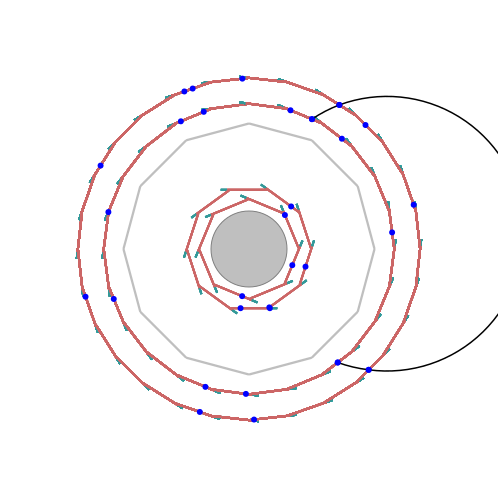
\includegraphics[width=.75\linewidth]{fig/tracking/s4.png}
      \caption{Figure showing an example of a 'floating' 4-hit track.}
      \label{fig:s4}
    \end{subfigure}%
    \begin{subfigure}{.5\textwidth}
      \centering
      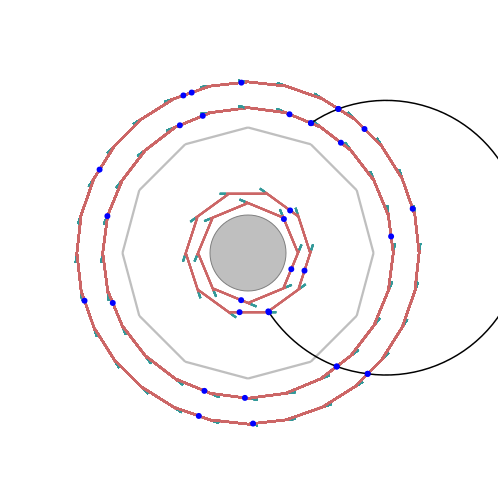
\includegraphics[width=.75\linewidth]{fig/tracking/s5.png}
      \caption{Figure showing the same floating 4-hit track that has been extended to a 5-hit track.}
      \label{fig:s5}
    \end{subfigure}
    \caption{The above figures show the detector in the x-y plane with an example track superimposed over. 
    In this, the above track is extended from a 'floating' 4-hit track to a 5-hit track. This is described as a floating 4-hit track as the track contains no hits in the innermost layer.}
    \label{fig:4_5}
\end{figure}
\subsection{Selection Cuts Applied to the 5 Hit Tracks}
Selection cuts must be applied to the 5 hit tracks in order to improve the purity. As there is a significantly larger distance that the particles are traversing between recorded hits in the detector, the fitting parameters must be less constrained as to allow a greater uncertainty due to multiple scattering.
\subsubsection{$\chi^{2}$ Minimisation}
Due to the lower fitting parameters of the 5 hit tracks, a four hit track that is being extended can be fitted multiple times, either with a triplet from a subsequent layer or a hit from the layer following. If the algorithm is successfully identifying a missing hit then only one of these generated tracks is correct.
By allowing a floating 4 hit track to run through all of the above methods and selecting the track with the lowest $\chi^{2}$ value, the purity is significantly increased.
\subsubsection{Propagation Cut}
For tracks where an individual hit is found, a cut is applied to find hits within a given window on a test layer.
\subsection{Effect on the Purity}
In this bit I want to talk about the number of tracks that have an inefficiency in a given test layer. The plot should show that the number of 5 hit tracks should be inverse to the test layer. Work in progress.
It currently shows there is a massive difference between the first layer and second. It also shows the purity to be rubbish in these sections.
\begin{figure}
    \centering
    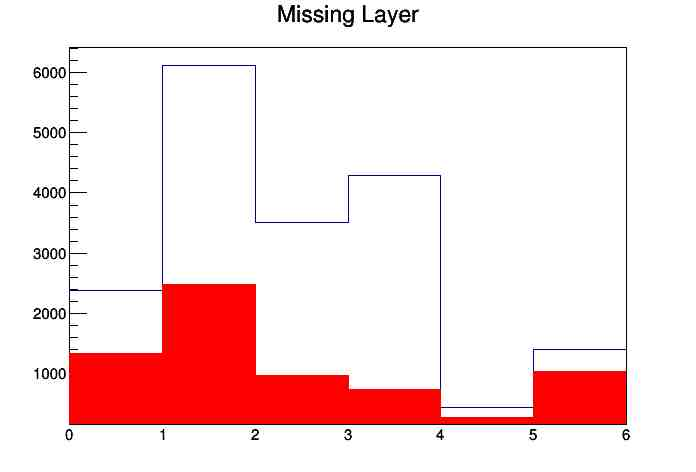
\includegraphics[scale=0.5]{fig/tracking/l.jpeg}
    \caption{Figure showing the number of 5 hit tracks and the inefficient layer that they are attached to. The red bar shows the number of pure tracks and blue shows the total number of tracks.}
    \label{fig:lay}
\end{figure}
\section{Validity of the 5 Hit Tracks}
\textbf{
    \begin{itemize}
        \item This should show the 5 hit tracks can be used.
        \item Discuss the momentum resolution with reference to the minimum resolution of tracks and compare to the 4, 6 and 8 hit track resolutions.
        \item This should also be where the proof that it can be used to vertex should be done.
    \end{itemize}
}
In this section, the use of five hit tracks is to be discussed. The purpose of the tracking is to accurately describe the trajectory of the decay products and calculate the respective momenta and energy.
By reconstructing the trajectory of tracks, vertices can be fitted to given decays and relevant frames can be saved to an offline database for further analysis. 
The secondary purpose of deriving the momenta of these tracks allows for background events to be rejected.
With these two purposes in mind, the assessment of the usefulness of these five hit tracks must be made using these two arguments. 
\subsection{Momentum Resolution}
The momentum of a track is calculated from the transverse curvature of the track and the linear projection along the z-axis.
Associated with the momenta of the tracks is a resolution calculation. This is based of the multiple scattering model provided and the number of layers a given track passes through.
For the purpose of this calculation, Monte Carlo information can be used to make a direct comparison.
\begin{equation}
    \sigma _{p} = \frac{p - p_{mc}}{p}
    \label{eq:res_mome}
\end{equation}
Equation \ref{eq:res_mome} describes the relation between the measured momentum of the track and the resolution of the measured momentum.
Where $\sigma _{p}$ is the resolution of the measured momentum, $p$ is the momentum of the particle in MeV and $p_{mc}$ is the true momentum.
In order to calculate the momentum resolution, equation \ref{eq:res_mome} was plotted as a function of measured momentum for each length of track.
An example of this plot is seen below in figure \ref{fig:resex}.
\begin{figure}
    \centering
    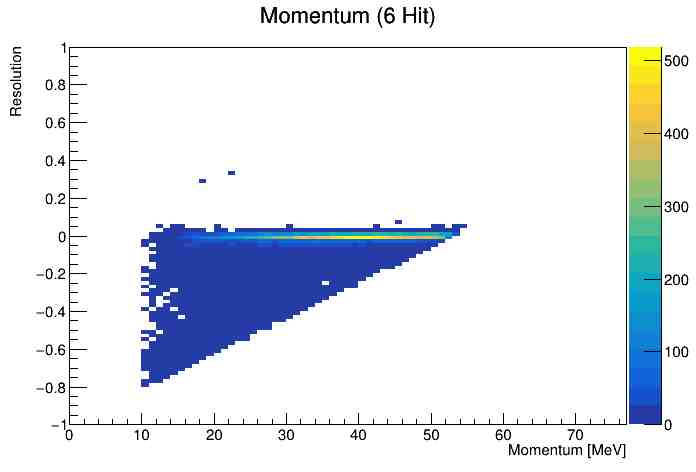
\includegraphics[scale=0.5]{fig/tracking/2dres.jpeg}
    \caption{Figure showing an example of the momentum resolution as a function of measured momentum.}
    \label{fig:resex}
\end{figure}
\par
1-dimensional slices are taken along the x-axis and the associated distributions are fitted with a crystal ball function.
The equation for the crystal ball fit is given below in equation \ref{eq:crysball}.
\begin{equation}
    f(x;\alpha,n,\bar x,\sigma) = N \cdot \begin{cases} \exp(- \frac{(x - \bar x)^2}{2 \sigma^2}), & \mbox{for }\frac{x - \bar x}{\sigma} > -\alpha \\
        A \cdot (B - \frac{x - \bar x}{\sigma})^{-n}, & \mbox{for }\frac{x - \bar x}{\sigma} \leq -\alpha \end{cases}
    \label{eq:crysball}
\end{equation}
From this fitting a mean is taken and an associated error on that mean is also calculated. By iterating this method over each momentum range and for each length of track distributions of the momentum resolutions can be plotted. 
This is shown in figure \ref{fig:resalt}. 
\begin{figure}
    \centering
    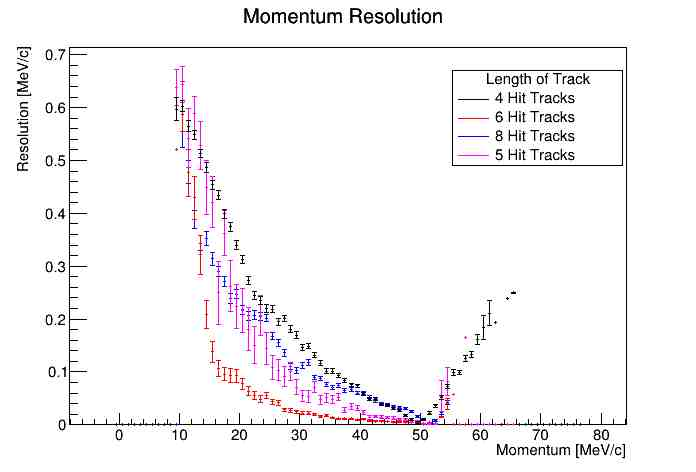
\includegraphics[scale=0.5]{fig/tracking/total_res_alt.jpeg}
    \caption{Figure showing an example of the momentum resolution as a function of measured momentum.}
    \label{fig:resalt}
\end{figure}
\section{Effect of Alternative Tracking}
\textbf{
    \begin{itemize}
        \item This should show the plots of hit efficiency and reconstruction efficiency.
        \item Discuss the difference between layers and why each layer responds differently.
        \item Should also include the effect on vertex reconstruction.
    \end{itemize}
}
\begin{figure}
    \centering
    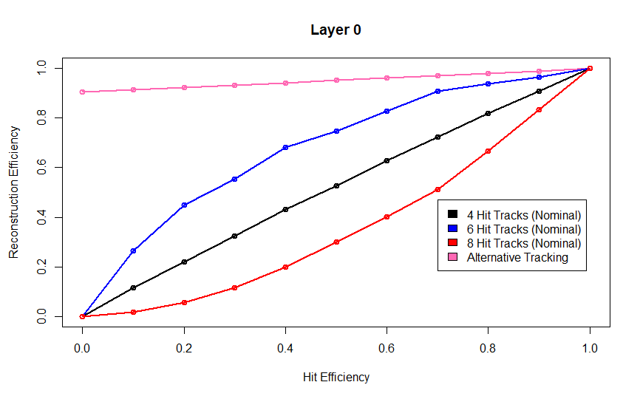
\includegraphics[scale=0.5]{fig/tracking/test_eff.png}
    \caption{Go figure.}
    \label{fig:eff5}
\end{figure}
\begin{figure}
    \centering
    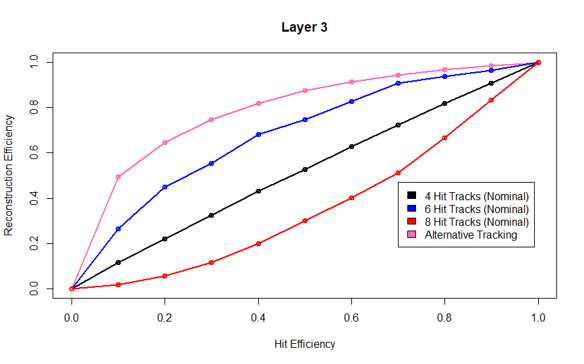
\includegraphics[scale=0.5]{fig/tracking/test_eff3.png}
    \caption{Go figure.}
    \label{fig:eff3}
\end{figure}
